\documentclass{IEEEtran}
\usepackage{graphicx}
\usepackage{amsmath}
\usepackage{cite}
\usepackage{booktabs}
\usepackage{fancyhdr}
\usepackage{graphicx}
\usepackage{biblatex}
\graphicspath{ {./Users/surajpowar/Downloads/alg_suraj_review/} }
\fancyhf{}
\renewcommand{\headrulewidth}{0pt}
\usepackage[
backend=biber,
style=alphabetic,
sorting=ynt
]{biblatex}
\addbibresource{alg_suraj.bib}

\rhead{Authors of Original Paper: Zakerolhosseini et al.}

\title{A Review on A Cryptosystem Based on the Symmetric Group Sn}
\author{Suraj Powar, \\
Clemson University, School of Mathematical and Statistical Sciences, South Carolina, USA 29631}
\date{\today}
\begin{document}
\maketitle

\thispagestyle{fancy}
\begin{abstract} The review is about the inclusion of theory of Symmetric Groups also known as $S_n$ groups from the class Math 6120.\\
The paper discusses about the implementation of concepts of cyclic group, disjoint cycles, and symmetric group $S_n$ to solve a public key problem to get the algorithm resistant to cyber attacks. This review will focus on how the concepts from group theory taught in class resonated with the foundational idea of implementation of algorithm by the authors.

\end{abstract}

\section{Introduction}
The paper proposed a public key system which used the theory of Symmetric groups $S_n$. They used an algorithm Pohlig Hellman \cite{pohlig2022improved} for cyber attack to check the resistance and to solve the Discrete Logarithm Problem which uses the algorithm to become resistant to the cyber attacks. Until the later years of 1970's the symmetric keys systems were used for transmission of messages in the cryptosystems. The basic fundamentals of a symmetric key cryptography is that two users who need to communicate to each other needs to posses a cipher or decipher the message. The logic was that without the key, it should be difficult to decipher the communications. The system which is known as a \textbf{public key} was essentially based on the exponential function of a finite field. This idea was inspired by abstract algebra concepts of having a finite field $GF(p)$ and also a generator g \(\in\) $GF(p)$. In the class we came across the concept couple of times, but we will be using the fundamentals of the finite fields and the generator rigorously in later section of the paper.  In the setup of the Diffie-Hellman key \cite{diffie1988first} exchange, suppose there are two users "A" and "B" wishes to agree upon a particular key, User "A" selects a random integer 2 \(\leq\) x \(\leq\) p - 2 and then transmits key $g^{x}$ to "B" over a public channel. User "B" also needs to select a random integer between 2 \(\leq\) y \(\leq\) p - 2, and then transmits $g^{y}$ to "A". Now according to the Diffie-Hellman key exchange, the users "A" and "B" having a common key $g^{xy}$ as we know from the concept of a finite field, the commutativity holds true, such that $g^{xy}$ = $g^{yx}$. Clearly this was efficient discrete logarithm algorithm to make less secure as it was easy to know for $(g^x)^y = g^{xy}$ then $g^{xy}$ was easy to compute. The difficulty of this problem is equivalent to computing the discrete logarithms as it is still unproven. \newline
There was another approach taken on the this problem by T. El-Gamal \cite{elgamal1985public}. The algorithm follows as Suppose $GF(q)$ is a known by public. The user "A" selects a generator g \(\in\) $GF(q)$, and an integer a. It then executes a public key, (g, $g^{a}$) as a public key and keeps it secret. The user "B" who requires to send a message say m \(\in\) $GF(q)$ to "A" selects an integer 2 \(\leq\) k \(\leq\) q - 2 randomly, which computes $m \cdot (g^a)^k = m \cdot g^{ak}$ and then sends a pair $(g^k, m \cdot g^{ak})$ to "A". The recovery is done by computing these equation. Now, based on the \textbf{Discrete Logarithm Problem (DLP)}, the authors from Teacher Training University and Shahid Beheshti University, Iran \cite{doliskani2008cryptosystem}, proposed a way which uses the symmetric groups properties in different ways that the approach mentioned above. They used the properties of group $S_n$ such as non commutative and used for high speed computing and increased flexibility in selection of keys that made the DLP algorithm resistant to attacks. \\
We shall see how they implemented in the next section of the review. \newline

\section{How paper is related to Math6120}
To relate the paper to the class syllabus that was taught during the semester in Math 6120, the idea of using the cyclic group G which were symmetric in nature and combining the generators for the field to explicitly form a discrete logarithmic function. We studied that Suppose G is a cyclic group, let the order of G be n so we know O(G) = n, and let \(\alpha\) and \(\beta\) \(\in\) G. The aim is to solve \[\alpha^x = \beta\]. Let us consider a field, say $GF(p)$ where p is a prime number. Assumption were made that \(\alpha\) is in $GF(p)$ is a generator of this field. Thus the function was created. Now to back this, we studied concept of permutation from the counting principles, which essentially uses the factorial notation to count the number of elements present in the symmetric group $S_n$. So $S_3$ will have 6 elements in it. The theorem they used was, \newline
\textbf{Theorem 2.1:} Every non identity permutation say \(\theta\) of $S_n$ can be uniquely expressed as a product of disjoint cycles of a length at least 2 \cite{herstein1975topics}. \newline
The follow up corollary was direct implementation of the concept that we studied in the class which enables to to find the order of disjoint cycles. \newline
\textbf{Corollary 2.2:} Let \(\sigma\) \(\in\) $S_n$ be the product of disjoint cycles say \(\theta_1\), \(\theta_{2}\), ..., \(\theta_{n}\) which \(\theta_i\) is an $m_i$ cycle, i = 1, 2, ..., k. Then the order of \(\sigma\) is $|\sigma|$ = lcm($m_!, m_2, ..., m_k$) \cite{rotman2015advanced}. \\
Another concept that was immensely used throughout the paper was that the factorials base systems. The authors used system that could be represented in the form of factorial base systems which was something that we studied in the class. The corollary was proposed as follows, \newline
\textbf{Corollary 3.2:} If a = $d_n \cdot d_{n-1} \cdot ... \cdot d_1$ is a number in factorial base systems the $d_n \cdot n! \leq a \leq (d_n + 1) \cdot n!$. This corollary was based on the foundational theorem which suggests every positive integer \(\alpha\) has a unique representation in a factorial base system. \newline
These concepts were used to develop the algorithm. The  output of the algorithm was competitive for computing the integer representation of $S_n$. The authors discovered that for $C_i$ = All the distinct i-cycle of $S_n$ then $A_{S_n} = \cup^{n}_{i = 1} C_i$. The $S_n$ is the regular symmetric group which is represented as $n!$. \newline
\textbf{Theorem 2.5:} For n \(\geq\) 2, \(\frac{A_{S_n}}{S_n}\) \(\leq\) 1 and $lim_{n \to \infty} \frac{A_{S_n}}{S_n} = 0$. \newline
I wrote a custom python script which confirmed the convergence of the integer representation of $S_n$. The curve which was suggested in the paper matched to the output I received. The figure below shows the output that was received from custom program. \newline
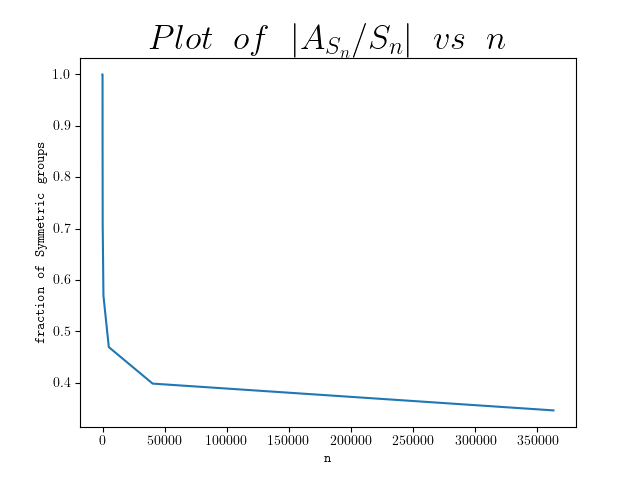
\includegraphics[width=9cm, height=7cm]{alg_suraj.png} \\
\textit{Fig 1: Vertical and horizontal axes show $\frac{|A_{S_n}|}{|S_n|} $ and n respectively.} \newline

\section{Conclusion}
The course of Abstract Algebra had lot of resonance in the paper. The authors led the foundational knowledge of cyclic group, symmetric groups and the other tools associated to group theory and implemented those in the algorithm. There is not much detail of algorithm mentioned in the review because it is simply out of the scope of the review with respect to the algebra class. But I would like to mention the outcome of the implementation as it did use the novel methods for implementation. The proposed system preserved the high security and the power, as the inclusion of $S_n$ group lead to the cryptosystems with much closer unconditional security than the current cryptosystems. The authors were able to perform the multiplication in $S_n$ which is composition of mapping for the n assignments in keys. The method was optimized for the exponentiation of keys using the non commutative and commutative multiplicative groups, which we did study a lot in class. The generator of the cyclic group \(\theta\) was generated very easily and it led to cost effective method so this scheme was resistant to attacks. \newline
The only negative feedback of the implementation of proposed algorithm was it was memory heavy. But they authors suggested that these can be extended to improvement of order of approximation for $O(n)$. It was very nice to know what we studied in the Math 6120 was being used in the real world research. I also got a chance to test the result by myself using custom program in python3.


\medskip


\printbibliography
\end{document}